% THIS IS SIGPROC-SP.TEX - VERSION 3.1
% WORKS WITH V3.2SP OF ACM_PROC_ARTICLE-SP.CLS
% APRIL 2009
% For tracking purposes - this is V3.1SP - APRIL 2009

\documentclass{acm_proc_article-sp}

% \usepackage[utf8]{inputenc}
% \usepackage[english]{babel} % English language/hyphenation
\usepackage{booktabs}
\usepackage{multicol}
\newcommand{\ra}[1]{\renewcommand{\arraystretch}{#1}}
\usepackage{float}
\usepackage{enumitem}
\usepackage{lipsum}
\usepackage{url}
\usepackage{svg}

\setlist[enumerate]
{nolistsep}

% references
% \usepackage[autostyle]{csquotes}
\usepackage[
  backend=biber,
  % style=alphabetic,
  citestyle=numeric-comp,
  % citestyle=authoryear,
  natbib=true,
  url=false,
  doi=true,
]{biblatex}
% \bibliography{ref}
\addbibresource{ref.bib}

\begin{document}

\title
{
	Gait Event Detection Using LSTM%
    \titlenote
    {
        We would like to thank the University of Pittsburgh's Human Movement
        Research Laboratory and its PI, Dr.~Gelsy Torres-Oviedo, for providing
        us with the motion capture data used for the experiments in this paper.
        The collection of these data was approved by the university's
        Institutional Review Board and all participating subjects gave prior
        consent to the use of their data for research purposes.
    }
}


\numberofauthors{3}
\author{
    % 1st. author
    \alignauthor
    Pablo A. Iturralde\\
        \affaddr{Bioengineering Department}\\
        \affaddr{University of Pittsburgh}\\
        \affaddr{Pittsburgh, PA}\\
        \email{pai7@pitt.edu}
    % 2nd. author
    \alignauthor
    Yin Zhong\\
        \affaddr{The Robotics Institute}\\
        \affaddr{Carnegie Mellon University}\\
        \affaddr{Pittsburgh, PA}\\
        \email{yinzhong@andrew.cmu.edu}
    \and
    % 3rd. author
    \alignauthor Jakob Bauer\\
        \affaddr{School of Computer Science}\\
        \affaddr{Carnegie Mellon University}\\
        \affaddr{Pittsburgh, PA}\\
        \email{jsbauer@andrew.cmu.edu}
}

\maketitle

\thispagestyle{empty}

\begin{abstract}
    In this paper, we propose a new data-based approach to gait event detection 
    using a Long Short-Term Memory Recurrent Neural Network.
    Our approach decisively outperforms existing methods such as the Foot 
    Velocity Algorithm and feed-forward Neural Networks with sliding window 
    in terms of the number of misclassified events and has a comparable 
    performance in terms of bias and variance for correctly classified events.
    Further advantages of our approach are that it does not rely on
    questionable heuristics and that it does not require heavy preprocessing 
    of the data.
    Given the promising initial results, we believe that it should be possible 
    to even further improve the current state of the art for data-based event 
    detection using a Long Short-Term Memory network.
\end{abstract}

\vskip 42em

\section{Introduction}
\label{sec:Introduction}

In order to study human gait,
it is necessary to divide the gait cycle into swing phase and stance phase.
The transition between the phases is marked by two events:
the subject's heel hitting the ground (heel strike) and the subject's toe
lifting off the ground (toe off).
It is paramount to accurately identify these events because otherwise, no
meaningful comparison of different stride cycles is possible.

% TODO introduce motion capture data

There are three basic approaches to event detection.
The first approach uses visual inspection to manually label the events.
Although quite accurate, the cost associated with this method is prohibitive for
all but the smallest amounts of data.
For this reason, it is not usually used as a stand-alone method but rather as a
postprocessing step for automated event detection systems or as a means to
generate small amounts of hand-labeled test data.
The second approach uses dedicated hardware such as force plates that measure
ground reaction forces and foot switches that are pressed when the foot is in
contact with the ground.
Due to their high accuracy, hardware-based methods are considered to be
state of the art for gait event identification.
However, their usefulness is limited by the fact that many laboratories do not
have access to the necessary equipment.
Furthermore, there is a risk of affecting the gait because some of the devices
require the modification of normal footware.
The third approach consists in automated event detection based solely on
the data.
If successful, this approach is superior to the other two because it scales
easily, does not require additional equipment and does not pose a risk of
affecting the gait.

Given these apparent advantages, it is not surprising that several data-based
methods have been proposed in the literature.
Although some of those methods achieve results that are accurate enough to be
useful in practice, they all have drawbacks such as relying heavily on
questionable heuristics or requiring an undue amount of data preprocessing.
For this reason, we present a new approach to gait event detection using a
Long Short-Term Memory (LSTM) recurrent neural network (RNN).
We believe that our method is superior to existing approaches both in terms of
accuracy and in terms of only requirying a small amount of training data and
preprocessing.

% TODO treat event detection as sequence labeling problem

This paper is organized as follows:
Section~\ref{sec:Previous Work}
discusses some of the existing data-based methods for event detection;
Section~\ref{sec:LSTM}
gives a short overview over LSTM networks in general;
Section~\ref{sec:Data}
contains a description the dataset;
Section~\ref{sec:Computational Resources}
shows states what computational resources were used for this project;
Sections~\ref{sec:Network Architecture} and \ref{sec:Network Training}
describe the architecture and training of our network;
Section~\ref{sec:Results}
presents the experimental results and compares them to existing baselines;
Section~\ref{sec:Conclusion and Future Work}
concludes and shows possible paths for future work.

\section{Previous Work}
\label{sec:Previous Work}

% \subsection{Heuristic Approach}
% \label{sub:Heuristic Approach}
\subsection{Foot Velocity Algorithm}
\label{sub:Foot Velocity Algorithm}

The Foot Velocity Algorithm (FVA)
\cite{OConnor2007}
belongs to a category of algorithms that use heuristics such as the velocity
and acceleration of heel and toe markers to detect motion events.
There are other examples of such algorithms, notably the one by Hreljac and 
Marshall
\cite{Hreljac2000}.
As these algorithms are quite similar, we will restrict our discussion
to the FVA.

The FVA takes as its input the location of the heel and toe markers as a
function of time.
After passing the data through a simple low pass filter,
a new virtual marker representing the foot center is created by taking the mean
of the heel and toe markers.
Finally, the velocity of this virtual marker is calculated.
Due to the quasi-periodic nature of walking, the graph of the velocity signal
exhibits a repeating pattern in which the toe off event is marked by a global
maximum and the heel strike by a local minimum.
This makes it possible to first detect the toe off event for each cycle and
then, in a second step, go through all the possible candidates for the heel
strike.
Using a constraint on the heel strike time, one of the candidates is selected
as the heel strike event.

% This makes it a popular choice in practice.
The FVA is widely used in practice.
The reason for the algorithm's popularity lies in the ease with which it can be
implemented:
it does not require any data preprocessing beyond some simple signal processing 
and it does not have to be trained.
That said, the FVA has several problems.
First, it makes questionable assumptions about the relationship between the
marker location and the gait cycle.
For instance, it is not clear that the marker velocity peaks exactly coincide
with the events to be identified.
Secondly, the algorithm is very sensitive to a threshold that has to be applied
in order to restrict the search for heel strike candidates.
The value of this threshold has to be manually tuned for each subject.
If not chosen carefully, the algorithm fails catastrophically.
Finally, the accuracy of FVA is bad when compared to more sophisticated methods
such as neural network and LSTM
(cf. Section~\ref{sec:Results}).

\subsection{Feed-Forward Neural Network}
\label{sub:Feed-Forward Neural Network}

\cite{Miller2009}
treats event detection as a classification problem and uses a classical
(feed-forward) neural network to perform the classification.
Each sample is classified individually based on a input window centered around
the desired sample.
At every time step, the window center is advanced by one sample
(so-called sliding window technique).
The use of a window allows to take into account the temporal dependencies
that exists between neighboring samples.%
\footnote
{
    Ideally, the window size should not be fixed but vary as a function of the 
    forward motion of the foot.
    The reason for this is that a fixed size window cannot guarantee that every
    window contains a sufficient amount of context because of the varying foot
    speed.
    For simplicity, we decided to use a fixed window size in our implementation
    of this method.
}

The input is not the actual motion capture data but rather position,
instantaneous velocity and instantaneous acceleration features extracted from
that data.
Furthermore, PCA is used to reduce the number of input variables from several
hundred to 50.
This dimensionality reduction is necessary because the number of inputs grows
linearly with the window size and the number of markers.

The network architecture itself is minimalistic: between an input layer
consisting of 50 input units and an output layer consisting of 2 units (one
for each leg) there is only one hidden layer with 33 sigmoid units.

The feed-forward neural network approach has several disadvantages.
In addition to heavy preprocessing consisting of feature extraction and PCA, the
data has to be split up into windows of variable length.
This in turn requires that the foot displacement be measured accurately from
the data which is non-trivial.
Moreover, the network architecture seems to be too simplistic to effectively
capture the long-range dependencies that exist between the data samples.

\section{LSTM}
\label{sec:LSTM}

Gait event detection can be seen as a form of sequence labeling (sometimes also
called segment classification), i.e., the task of assigning a sequence of labels
(swing phase vs. stance phase) to a sequence of input (motion) data.
The success of a sequence labeling system hinges on its ability to
incorporate context information from both sides of the segment in question.
%
One way to incorporate this context information is to use feed-forward or
recurrenct neural networks with a sliding windows (as in the case of
\cite{Miller2009}).
However, as the range of useful context and thus the required window size is in
general not known in practice, this approach is only of limited usefulness
\cite{Graves2012}.

A second approach consists in using a RNN and passing the
input sequence forwards and backwards to two separate hidden layers that are
connected to the same output (so-called bidirectional networks
\cite{Schuster1999}).
The issue here is the vanishing gradient problem that causes the influence of a
given input to either decay rapidly or to blow up exponentially
\cite{Hochreiter1991}.

A third approach is LSTM.
An LSTM network is an RNN where the summation units in the hidden layer are 
replaced with so-called memory blocks.
These blocks consist of a memory cell as well as three multiplicative units 
called input gate, output gate and forget gate.
By controlling these gates, it is possible to store information in the memory 
cell for long periods of time
\cite{Graves2012}.
LSTM is theoretically superior to both the window method and the bidirectional 
networks as does not require the use of a window and does not suffer 
from the vanishing gradient problem.
It has also successfully been used in practice for tasks that require long range 
memory such as speech recognition 
\cite{GravesSchmidhuber2005}
and handwriting recognition
\cite{Liwicki2007}.
Given these advantages, we decided to use LSTM for our gait event detection
system.

\section{Data}
\label{sec:Data}

\subsection{Collection}
\label{sub:Collection}

Our training and testing was conducted on data from 10 healthy subjects walking 
on a treadmill at three different speeds for 50 seconds. Each sequence of 50 seconds is called a trial. This amounts to a total of 1500 seconds of recorded data, which roughly correspond to 1000 gait cycles.  For each subject, 3D motion capture data was collected using 18 reflective markers placed at precise body locations.%
\footnote
{
    The locations used were toe, ankle, heel, knee, greater trochanter (hip), tibia, femur, and anterior and posterior superior illiac spine (pelvis) on each leg.
}
The sampling frequency of this data is 100Hz. The event labels (target) were computed from ground force reaction data from force sensors embedded in the treadmill 
which is considered the gold standard in the field. 
In order to compute events the ground reaction forces in gravity's axis are thresholded at 20N; whenever the forces exceed this threshold, the foot is considered to be on the ground (stance). By searching for the transitions between stance and no-stance, the events are found.
The sampling frequency of this data is 1kHz.

\subsection{Test/Training Split}
\label{sub:Test/Training Split}

The data was separated into a training and a testing set in two different ways. Dataset 1 takes the first 25 seconds of data from each trial as the training sample, and the following 25 seconds as the testing sample. This dataset was meant to test how well a trained network can generalize to new gait cycles, given that it was trained on data including the same subject and walking speed. As such, it is the most basic test of performance that can be done. Dataset 2 includes the same data, but splits it along trials: all 50 seconds of 15 trials were used for training, and the remaining 15 trials were used for testing. It is worth noticing that this second dataset necessarily has different subjects in its training and testing sets, so it allows us to assess how the algorithm generalizes to new users without being trained on them.

\subsection{Preprocessing}
\label{sub:Preprocessing}

We used the following preprocessing steps:
\begin{enumerate}
 \item The data was translated so that the mid-hip position (average position of the left and right hip markers) is located at $(0,0,0)$ at all times.
 \item The data was rotated so that gravity is aligned with the $z$ axis (was already the case) and the $x$ axis is aligned with the vector going from the left hip marker to the right hip marker, projected onto a plane orthogonal to $z$. The $y$ axis is defined as the direction orthogonal to $x$ and $y$. This allows the data to be independent of walking direction and the absolute reference frame in which the data was captured.
 \item The data for each marker was standardized.
\end{enumerate}

% TODO explain motion capture data either here or in introduction

\section{Computational Resources}
\label{sec:Computational Resources}

Our LSTM implementation is written in Torch, a scientific computing framework 
for LuaJIT.%
\footnote
{
    See 
    \url
    {
        torch.ch
    }
    for detail.
}
The network was run on an Amazon EC2 instance of type g2.2xlarge.
This instance type comes with an 8 core 2.6 GHz Intel Xeon E5-2670 processor and 
an Nvidia GRID K520 GPU that is composed of two 4 GB GK104 GPUs.

\section{Network Architecture}
\label{sec:Network Architecture}

We took an iterative approach to build our neural network. Initially we implemented a low-complexity LSTM network, evaluated its performance by cross-validation, then attempted to improve its performance and robustness by adding further components one at a time while evaluating performance.

\subsection{Initial Design}
\label{sec:arch-simple}

The first iteration of network has 3 layers: input, LSTM (hidden), and output. Input is presented to the network in the form given (transformed coordinates of markers), while output (state of legs) is presented as ``one-hot'' vectors. The LSTM layer consists of several memory blocks, each containing only one cell (i.e. gates are not shared between cells). The output layer employs standard soft-max activation function, which is matched with negative-log-likelihood loss function. The only model hyper-parameter is the number of LSTM cells. In this setup, the LSTM layer learns to model features in the underlying human-treadmill dynamic system, while the output layer uses these features to emit belief of leg state at each timestep.

While this is a very simple architecture, it allows rapid training, and already achieves similar or even better performance on our testing datasets compared to baseline algorithms. However, its performance often stops improving very early and we cannot control for overfitting, given the insufficient regularization.

Because of time constraints, this architecture is the only one we managed to train and test thoroughly. All of the results presented in this report stem from the use of this architecture. However, we managed to implement some improvements for future test that are described next.

\subsection{Improvements}

Our initial design employs a fairly wide LSTM layer for our data volume. In order to make full use of each cell and prevent overfitting from co-adaptation between LSTM cells, we inserted a \emph{dropout} \cite{Hinton2012} layer between input and LSTM layers. While dropout was initially proposed for use in feed-forward networks, it has been used extensively in RNN featuring LSTM cells to great success \cite{Pham2013}. Its major advantage over other approaches is that only one additional hyper-parameter (dropout probability $p$) needs to be tuned. Its biggest drawback is slower convergence.

Another commonly used approach to improve robustness and convergence rate is to replace activation functions of some sigmoid neurons with ReLU (rectified linear unit). Because the sigmoids in LSTM serve special functions (``gating''), they cannot be readily replaced. Instead, we can incorporate ReLU by inserting an additional hidden layer between dropout layer and LSTM layer, which also serves the function of learning coordinate transformations. In addition, ReLU works well with dropout in practice \cite{Pham2013,Dahl2013}. The hidden layer introduces one additional hyper-parameter (layer size).

In an attempt to further improve performance, we replaced the single LSTM layer with two LSTM layers connected back-to-back. In order to avoid gradients vanishing in the input-side LSTM layer, we removed the output sigmoid from traditional LSTM cells as described in \cite{Gers2002}. However, the addition of a recurrent layer has great impact on difficulty of training. An variation of this architecture which merges the two LSTM layers (2nd-order LSTM-like RNN) might be able to solve this problem \cite{Monner2012}.

\section{Network Training}
\label{sec:Network Training}

% \subsection{Parameter search}
Initially we wanted to determine what values to use for the training of our network to achieve the best possible performance. In order to do this, we trained our network for a few epochs (10) with a  number of different parameters to see its performance.
For each parameter set, we ran the training three times, in order to average among the realizations and obtain results less susceptible to the initial conditions.
All results from this section used the training half of Dataset 1, and training was implemented as stochastic gradient descent (SGD), with each datapoint corresponding to a sequence length of 500 samples (5 seconds).

\begin{figure}[H]
 \centering
 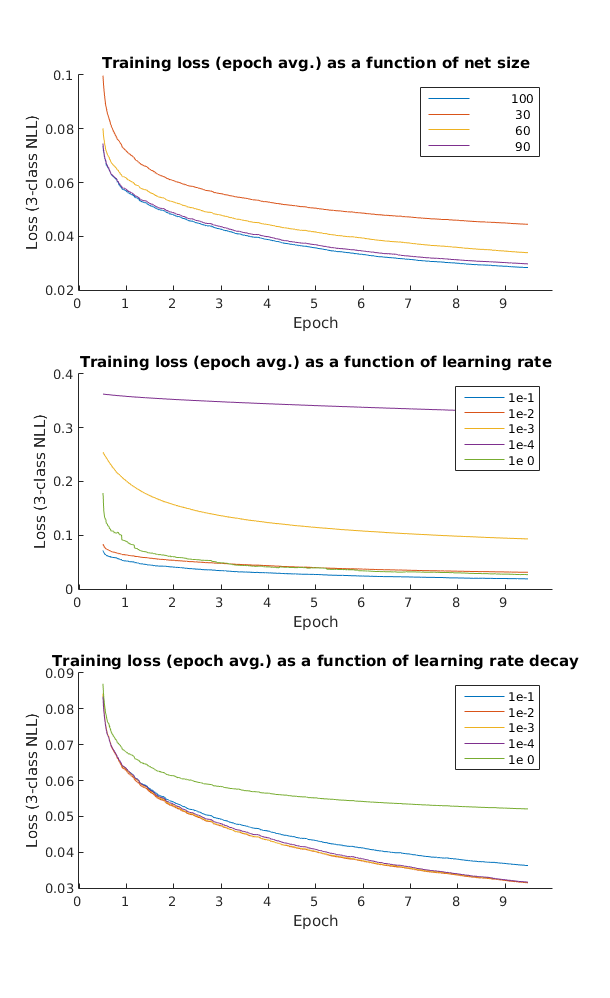
\includegraphics[scale=.55]{./figures/parameterSearch.png}
 % parameterSearch.png: 0x0 pixel, 300dpi, 0.00x0.00 cm, bb=
 \caption{Convergence of the network in the first 10 epochs as a function of different parameters.}
 \label{fig:paramSearch}
\end{figure}

As can be seen from Figure \ref{fig:paramSearch} a good learning rate was about $1e-1$ and an appropriate decay was about $1e-2$ (learning rate decay was automatically implemented by the \textit{adagrad} method of Torch's \textit{optim} toolbox as inversely proportional to number of iterations, here $1e-2$ means it takes 100 epochs for the learning rate to decay to half its initial value). Although an ideal network size cannot be inferred from here, we can see the decreasing returns on adding additional units to the network. We decided to use a network of 100 cells for further testing. However, the computational resources from the Amazon EC2 instance allows for training of networks of much larger sizes well above 1000 cells.

\section{Results}
\label{sec:Results}

\subsection{Dataset 1}
Once we settled on parameters for our network, we trained it for 100 epochs and tested it on dataset 1. We compared results from Miller's feed-forward network, O'Connor's heuristic and our LSTM network. We assessed the results as follows: if a detected event was less than 100ms apart from the actual event (ground truth derived from force-plates), we measured the difference in times and quantified it in a histogram. If the detected event was more than 100ms apart from the closest true event, we consider it a false positive. In the same way, if no event was detected within 100ms of an actual event, we consider it to be a false negative. All four possible events (left heel-strike, toe-off, right heel-strike and toe-off) were considered independetly.  Results are summarized on figure \ref{fig:halfAndHalfTrials}. Each plot represents the histogram of time differences between actual and detected events when they are within a 100ms window of each other. At the top of each plot appear the total number of false positives (fp) and false negatives (fn) for each of the methods compared. O'Connor's results were very poor compared to other methods (larger bias and variance), so they were excluded from the figure. The three methods that appear in the figure are: Miller with the default parameters (33 hidden units), LSTM network of 100 units trained over 30 or 50 epochs, to show the convergence. From this figure we can see that performance of all three algorithms in terms of bias ($\mu$) and standard deviation ($\sigma$) is comparable. However, the LSTM network performs better in terms of false negatives and false positives, with almost no bad detections or missed events, while Miller's has a significant amount of false positives especially.\\


\begin{figure}
 \centering
 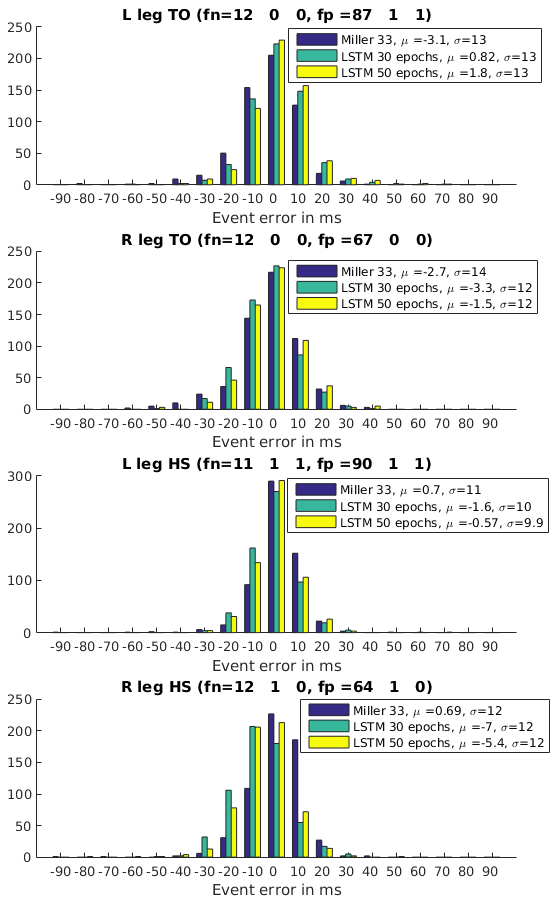
\includegraphics[scale=.45]{./figures/Test1_2Train1_1Compare.png}
 % \includesvg[scale=.31]{./figures/Test1_1Train1_2Compare.svg}
 % Test1_1Train1_2Compare.png: 0x0 pixel, 300dpi, 0.00x0.00 cm, bb=
 \caption{Comparison of Miller vs. LSTM network for various training intervals, for dataset 1.}
 \label{fig:halfAndHalfTrials}
\end{figure}

\subsection{Dataset 2}
The second dataset was designed to assess how well the methods generalize to new users. We performed the same treatment as for the previous dataset, and results are shown on \ref{fig:halfAndHalfUsers}. From these results we can see that the LSTM network achieves better accuracy than Miller, with less false positives and false negatives. However, the false positive rate is somewhat high for the LSTM network too. It can also be seen that for the LSTM network trained over 50 epochs that some overfitting is happening, as the number of false positives increases noticeably, and accuracy is also slightly reduced. We didn't implement any way to prevent over-fitting, so this is not too surprising. Perhaps it is good news that 30 epochs of training suffice to achieve the network's optimal performance.

\begin{figure}
 \centering
 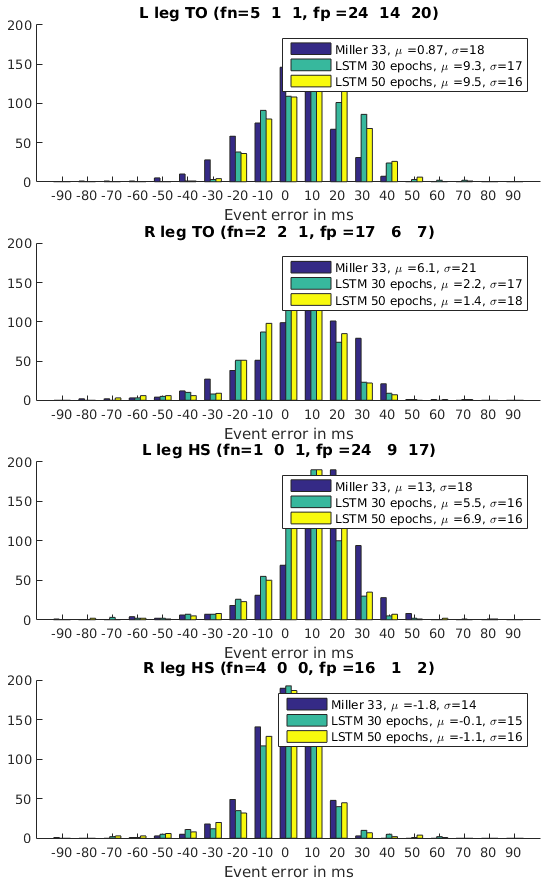
\includegraphics[scale=.45]{./figures/Test2_1Train2_2Compare.png}
  %\includesvg[scale=.4]{./figures/Test2_2Train2_1Compare.svg}
 % Test1_1Train1_2Compare.png: 0x0 pixel, 300dpi, 0.00x0.00 cm, bb=
 \caption{Comparison of Miller vs. LSTM network for various training intervals, for dataset 2.}
 \label{fig:halfAndHalfUsers}
\end{figure}

\section{Conclusion and Future Work}
\label{sec:Conclusion and Future Work}
\subsection{Conclusions}
The results from our initial implementation of the LSTM network are very encouraging. Compared to the baseline methods, we achieved less confusion (false positive and false negative rate) and similar or better accuracy, measured through bias and quadratic error. O'Connor's heuristic performed very poorly, with biases and standard deviations tens of milliseconds larger than what Miller and the LSTM network achieved. This is not too surprising since O'Connor is a fixed heuristic method with no way to adapt to the data (requires no training).

Miller performed much better than O'Connor but we still found that LSTM performed slightly better. In \cite{Miller2009} the reported results for the method are similar (although slightly worse) than what we found here for the same algorithm. However, \cite{Miller2009} only uses 72 gait cycles (total) for his training, which is a lot smaller than our dataset. Miller also fails to discuss his cross-validation method and false detection rates, so it is not clear whether the high false positive rate was an issue for him or whether it is an artifact of our implementation and the larger dataset we tried to train on. Miller did achieve his performance including subjects with pathological gait, but given the small dataset, it is hard to say how many of his samples were really pathological and how much that affected performance.

It is worth noticing that our implementation can do event detection in real time, both in the sense that it is computationally tractable and that our prediction is causal, relying only in past marker data. This makes our method unique, as we couldn't find anything in the literature that offered similar guarantees. Overall, the results we obtained are satisfying and we expect to polish them a little further before submitting them for publication in a gait research journal.

\subsection{Future work}
Although our results are promising and seem to improve the current state-of-the-art, there a few things that still can be done to assess and improve performance:
\begin{enumerate}
 \item Run a true grid search to find the best training parameters.
 \item Run the training for a longer time and use cross-validation to determine reasonable stopping criteria and avoid over-fitting.
 \item Use the network with a delay in the output, so we effectively use information of a window of time around the desired time sample to infer events. This would make this method more comparable to the exisiting algorithms, which usually work with the smoothing problem, and not with the real-time filtering problem. Arguably this could only improve the performance of the method, as more information would be available to make the classification of each sample.
 \item Assess generalization to pathological gait subjects.
 \item Assess generalization to over-ground walking data (no ground truth in our dataset).
 \item Investigate possible pre-processing to guarantee that method is invariant to walking speed, and subject height and weight.
 \item Study possible modifications to make the network truly invariant to the left/right symmetry. Currently the network is trained to output events for both legs with marker data from both sides of the body, but we know that the symmetry of the problem could be exploited further. However, this could prove to be an issue on subjects with highly asymmetrical gait.
 \item Incorporate prior information from the transitions that occurr during gait. In normal walking the events happen in a pre-established order (left heel-strike - right toe-off - right heel-strike - left toe-off) which gives us some information on the possible upcoming transitions based on the current state. While we can speculate that a recursive NN learns this with training, we could incorporate this information for better accuracy during normal walking conditions.
 \item Reduce the number of markers used to achive performance. While ours is a rich dataset, not all  motion-capture datasets will include all the markers used. Furthermore we can expect the feet markers to contain the most information about the events, while other markers may be more easily discarded.
\end{enumerate}


% \section{Data}
% For the initial training purposes, we selected data from 8 healthy subjects walking in a treadmill at three different speeds for 100 seconds each. Additionally, we took data from 13 stroke subjects, walking at a single speed for 100 seconds. For each subject, the input data is 3D marker position of 18 different markers placed in the same anatomical positions for each subject, sampled at 100Hz. The event labels (target) were computed from ground force reaction data samples at 1kHz for healthy subjects, and 2kHz for stroke subjects. This is currently considered the gold standard \cite{miller_gait_2009,miller_gait_2009,Hreljac2000}. \\
% %The problem is then to classify each sample in time as one of four different classes: both feet in contact with the ground, both feet off the ground, left feet only on the ground and right feet only on the ground.
% \section{Algorithms}
%
% \section{Computational Resources}
%
% For the LSTM network we are using
% an Amazon EC2 instance of type g2.2xlarge.
% This instance type comes with an 8 core 2.6 GHz Intel Xeon E5-2670 processor and an Nvidia GRID K520 GPU that is composed of two 4 GB GK104 GPUs.
% We chose Torch as our computing framework.
%
% \section{Intermediate Results}
% We implemented and tested the two methods described in \cite{oconnor_automatic_2007} and \cite{miller_gait_2009}. Results are in line with the ones presented on each paper. Summaries of the true error (detected event time minus actual event time) can be found in Figures~\ref{fig:oconner} and \ref{fig:miller}.
% There are no results yet for the LSTM approach.
%
% \section{Difficulties and Future Work}
% In the following weeks we will be implementing an LSTM network on Torch. As we have no experience using Torch in the past, we are not sure how long it will take.\\
%
% Other future work includes feature engineering to determine the most relevant input variables, from all the available marker position data and its derivatives, in order to reduce the size of the network that has to be trained. We would also like to extend the capabilities of the method to data that was acquired in natural walking (as opposed to treadmill walking). We believe adequate feature engineering may be enough to achieve this objective too.\\

\printbibliography

% \appendix

\end{document}
